\begin{figure*}
\centering
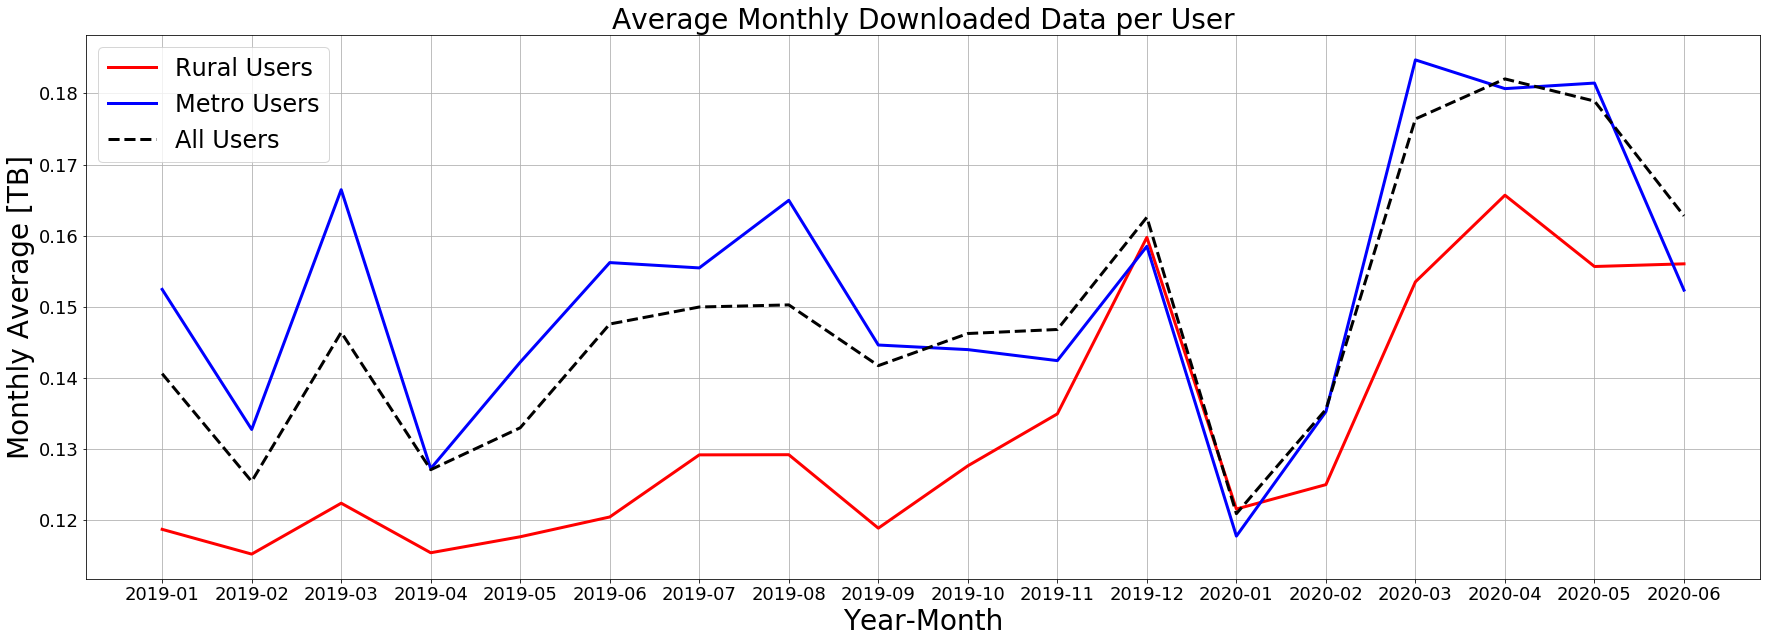
\includegraphics[width=1.0\linewidth]{figs/monthly_downloaded_data.png}
\caption{Graph showing the average consumption of downloaded data per user from 2019 to June 2020, partitioned by user county population.}
\label{fig:downloadmetro_rural}
\end{figure*}

\subsection{Analysis of Data Usage by Population Demographics}

\subsubsection{Average Monthly Usage}
A high-level overview of the effect of COVID-19 on internet usage can be seen by analyzing the average monthly downloaded data per user. As evidenced in Figure \ref{fig:downloadmetro_rural}, we notice a sizable increase in overall downloaded data in the months of March, April, and May. This increase is consistent across both county population levels, although it is more pronounced in metro areas: the 3 largest months by downloaded data occurred in the first 3 months of the pandemic. In rural areas, only one pandemic month is higher than December $2019$ levels.

Interestingly, in the fourth month of the pandemic, we notice a drop in overall downloaded data in metro areas, while rural areas remain constant. This drop coincides with the relaxation of many stay-at-home orders, indoor dining bans, and curfews in cities across America \cite{money2020la}, \cite{gov2020nyc}. 

\begin{figure*}
\centering
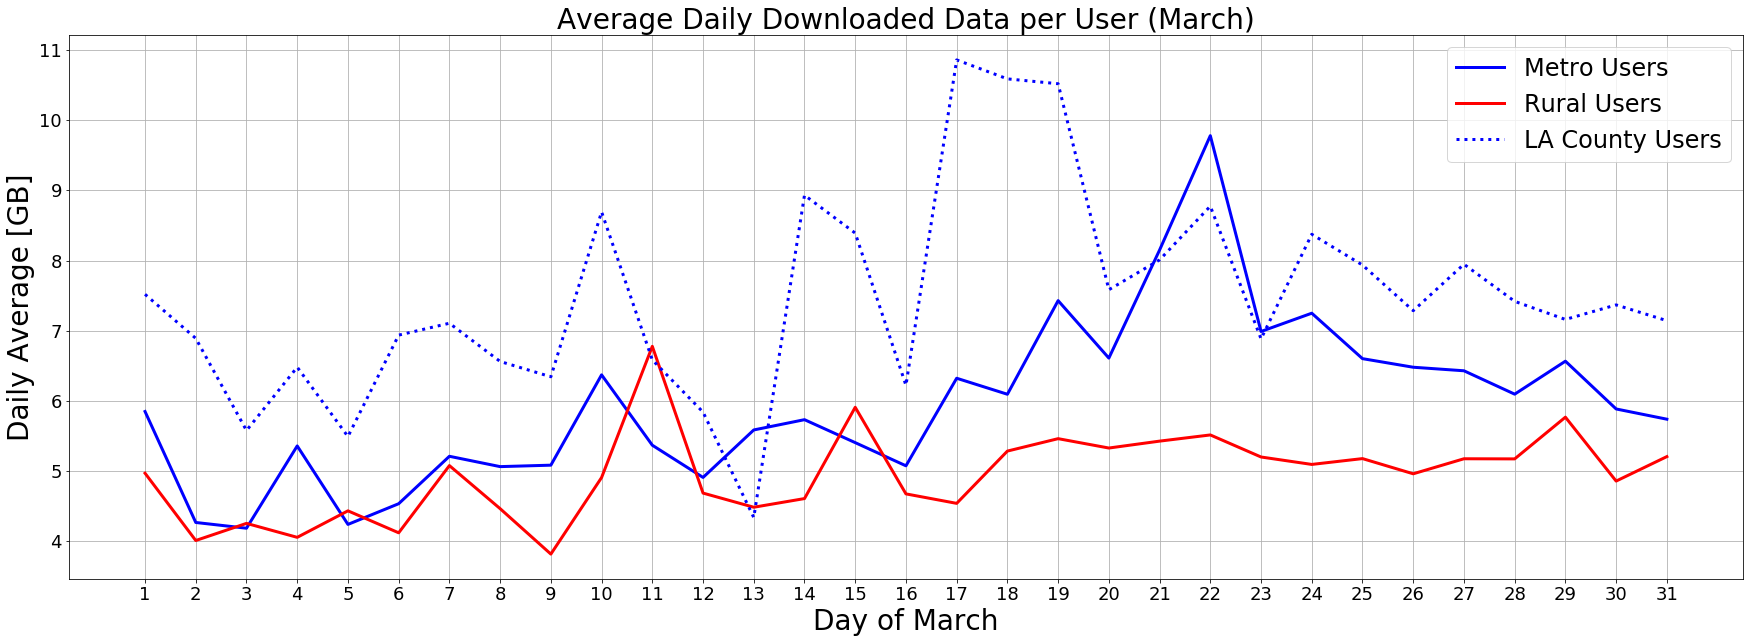
\includegraphics[width=1.0\linewidth]{figs/daily_downloaded_data.png}
\caption{Graph showing the daily consumption of downloaded data per user in March 2020 for those in metro and rural areas, as well as LA county.}
\label{fig:dailymetro_rural}
\end{figure*}

\subsubsection{Daily Data Usage}
We can take a higher resolution approach to the analysis of downloaded data usage by analyzing daily averages. We focus specifically on the month of March because of the placement of various stay-at-home orders, school shutdowns, and curfews at both the national and local levels. On March 16 \cite{trump2020coronavirus}, the White House issued a social distancing recommendations for the entire country. Following this announcement, we observe that users in metro areas use a significantly larger amount of data than those in rural areas. In the first half of the month, there was no such difference (Figure \ref{fig:dailymetro_rural}). This is a predictable result: as metro areas were hit harder by the early weeks of the pandemic than rural areas, adherence to stay-at-home guidelines would likely have been followed more stringently. 

We can additionally look at data usage patterns within counties, allowing us to correlate usage patterns with local ordinances. Los Angeles (LA) county has the most users in the MBA dataset ($n=44$), so we examine the daily average downloaded data per user for all those residing in LA (Figure \ref{fig:dailymetro_rural}). We observe the first large spike on March $14$, the day after many schools in the county shutdown \cite{haire2020LA}. We also notice a larger spike in the days following the national stay-at-home order. We should note that March $14$ was a weekend, so the spike we observe is not due to remote learning, but is instead likely due to people seeking entertainment from the internet over outside options. 

